\documentclass[12pt]{extarticle}

% Language setting
% Replace `english' with e.g. `spanish' to change the document language
\usepackage[english]{babel}
\usepackage[
    backend=biber,
    bibstyle=ieee,
    citestyle=numeric,
]{biblatex}
\addbibresource{cite.bib} %Imports bibliography file
\usepackage{soul}
\usepackage[export]{adjustbox}
\usepackage{listings}
\usepackage{makecell}
\usepackage{longtable}
\usepackage[table,x11names]{xcolor}
% Set page size and margins
% Replace `letterpaper' with`a4paper' for UK/EU standard size
\usepackage[letterpaper,top=2cm,bottom=2cm,left=3cm,right=3cm,marginparwidth=1.75cm]{geometry}

% Useful packages
\usepackage{amsmath}
\usepackage{graphicx}
\usepackage{subcaption}
\usepackage[colorlinks=true, allcolors=blue]{hyperref}
\usepackage{textcomp}

\title{
    Pretext Tasks: \\
    can they make models more robust?
}
\author{Artem Sereda artem.sereda@campus.tu-berlin.de}

\begin{document}
    \maketitle

    \begin{abstract}
    The continuous improvements in the image classification over the recent years are opening doors to
    a lot of life-changing applications of Machine Learning (ML).
    It has been proven that including a pretext task improves classifiers' standard accuracy.
    Despite numerous studies of an adversarial vulnerability phenomenon, there is no clear answer
    how a choice of pre-training influences Neural Networks' (NNs') adversarial robustness.
    This paper will first give a general introduction to white box adversarial attacks using Fast Gradient Sign Method (FGSM),
    as well as to some popular pretext tasks.
    Afterwards the impact of including a pretext task, as well as its choice will be evaluated.
    The implementation of the evaluation for this paper can be found in accompanying GitHub repository~\cite{github}.
    \end{abstract}


    \section{Introduction}

In recent years, neural networks have had a lot of success in image classification.
This has led to advances in many areas, including computer vision and object recognition.
A.e.advances in a constantly ongoing ImageNet classification challenge, which were achieved
through new approaches,
rather than increasing NN number of layers and parameters~\cite{russakovsky2015imagenet,DBLP:journals/corr/abs-1905-11946}~.
However, neural networks are also vulnerable to adversarial attacks~\cite{ilyas2019adversarial}.
Adversarial attacks are designed to fool neural networks into misclassifying data.
This can have serious consequences, as it can lead to incorrect results or decisions.
Typical approach to ensure robustness, would be adversarial training, however if often comes with a cost of
reduced classification accuracy~\cite{https://doi.org/10.48550/arxiv.1805.12152}.
Pretext tasks had shown themselves to be usefully in improving accuracy~\cite{kolesnikov2019revisiting}.
In this research, I would like to evaluate how including state-of-the-art pretext tasks in the training process
influences neural networks' vulnerability to adversarial attacks.

\subsection{Background}

\paragraph{Adversarial attack}
Goodfellow defined adversarial attacks as “inputs to machine learning models that an
attacker has intentionally designed to cause the model to make a mistake.”
~\cite{DBLP:journals/corr/abs-1802-08195} \\
In the domain of image classification, adversarial attacks are images usually formed by applying a small perturbation
(which is barely noticeable for human viewer) to a naturally occurring image, with intention to make NN miss-classify.
There are many types of adversarial attacks,
and the type of attack depends on the type of model that is being attacked.
In this paper, I focus on the white-box attack, where the attacker has full access to the model and its parameters,
namely Fast Gradient Sign Method.

\paragraph{Fast gradient sign method}
This method was first introduced by Goodfellow and Jonathon Shlens and Christian Szegedy
~\cite{goodfellow2015explaining}.
It produces adversarial images which make NN miss-classify,
but are still recognisable as of the same class for human viewer.
Fast gradient sign method (further denoted as FGSM) works
by using the gradients of the neural network to create an adversarial pattern.
For an input image,
the method evaluates the signed gradient of the loss function with respect to the input image to create a pattern,
which maximises the loss.
The pattern is then added pixel wise to original image.
The new image is called the adversarial image.
The process can be summarised using the following expression:
\begin{equation}
    adv\_x = x + \epsilon \cdot sign(\nabla_x J(\theta, x, y))
\end{equation}
(where $\epsilon$ denotes the intensity of adversarial pattern).
\\
\begin{figure}[h]
    \begin{subfigure}{0.4\textwidth}
        \caption{Tulips 40\% confidence}
        
\includegraphics[width=8cm]{images/og_image}
    \end{subfigure}
    \begin{subfigure}{0.4\textwidth}
        \caption{Adversarial pattern for this image}
        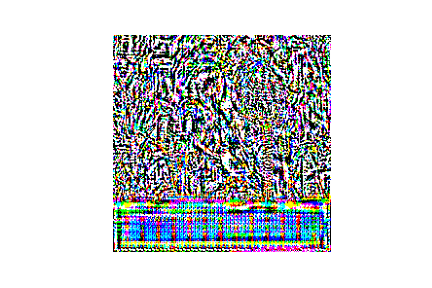
\includegraphics[width=8cm]{images/adv_pattern}
    \end{subfigure}
    \\
    \begin{subfigure}{0.4\textwidth}
        \caption{$\epsilon = 0.01$, Roses 40\% confidence}
        
\includegraphics[width=8cm]{images/adv_attack_001}
    \end{subfigure}
    \begin{subfigure}{0.4\textwidth}
        \caption{$\epsilon = 0.1$, Roses 40\% confidence}
        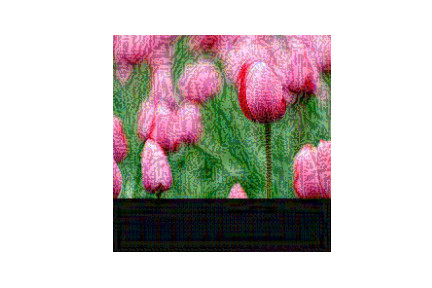
\includegraphics[width=8cm]{images/adv_attack_01}
    \end{subfigure}
\end{figure}

\paragraph{Pretext task}
Pretext task is the self-supervised learning task solved to learn visual representations,
with the aim of using the learned representations or model weights obtained in the process, for the downstream task.
It has been showm, that pretext tasks can significantly improve NNs accuracy.~\cite{kolesnikov2019revisiting}
It is also believed they contribute to NNs learning of important (as per human agents) features.
In this paper I focus on rotation and jigsaw pre-text tasks.

\paragraph{Rotation pretext task}
A common choice of pretext task could be to produce 4 copies of
a single image by rotating it by {0°, 90°, 180°, 270°} and let a single network predict the rotation which was applied.
Alexander Kolesnikov and Xiaohua Zhai and Lucas Beyer: "Intuitively, a good model should learn to
recognize canonical orientations of objects in natural images" ~\cite{kolesnikov2019revisiting}.

\paragraph{Jigsaw pretext task}
The task is
to recover relative spatial position of 4 sampled image patches
after a random permutation of these patches was performed.
~\cite{kolesnikov2019revisiting}
All of these patches are concatenated in 'puzzle' image,
which is later sent through same network, which needs to predict a permutation applied.



\section{Methods}

\paragraph{Model}
Convolutional networks' architectures for image recognition have evolved quite drastically in recent years,
with numerous options available "out of the box".
A.e.\ Efficient Net (further denoted as EffNet) delivers impressive accuracy,
while being able to scale better than a lot of previous architectures~\cite{DBLP:journals/corr/abs-1905-11946}.
For this paper, the evaluation was done using it, namely EfficientNetB0
\footnote{For details about EfficientNet usage please refer to \href{https://keras.io/api/applications/efficientnet/}{keras/efficientnet}}.

\paragraph{Rotation pretext task}
Each image from original dataset was rotated 0°,90°,180°,270° and assigned new pseudo label from 0,1,2,3 accordingly.
All 4 batches of rotated images were concatenated in dataset, and shuffled.
Then the last dense layer of NN was replaced with a dense layer for the corresponding number of pseudo classes (4).
Then the same model was then trained to identify rotation applied.
\begin{figure}[h]
    \begin{subfigure}{0.33\textwidth}
        \caption{Label = 0}
        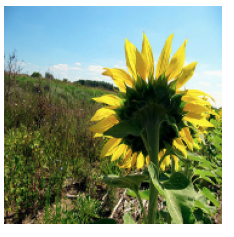
\includegraphics[width=5cm]{images/rot_0}
    \end{subfigure}
    \begin{subfigure}{0.2\textwidth}
        \caption{Label = 1}
        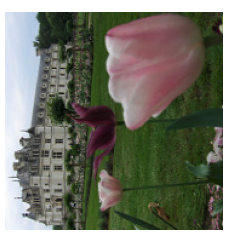
\includegraphics[width=5cm]{images/rot_1}
    \end{subfigure}
    \begin{subfigure}{0.33\textwidth}
        \caption{Label = 2}
        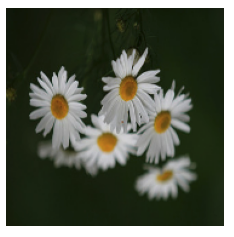
\includegraphics[width=5cm]{images/rot_2}
    \end{subfigure}
    \caption{An example how images used for rotation pretext task could look like}
\end{figure}




\paragraph{Jigsaw pretext task}For jigsaw,
a similar approach as described by Mehdi Noroozi and Paolo Favaro~\cite{DBLP:journals/corr/NorooziF16} was adopted.
Random 4 out of 24 possible permutations were chosen for each batch (number of possible permutation can be obtained from Newtonian binomial $P=\frac{r!}{(r-n)!}$).
For each permutation, each image was cut in 4 equal parts,
afterwards these tiles were permuted according to chosen permutation, and concatenated in 1 (puzzle) image.
Similarly, to rotation pseudo labels in [0\ldots23] had been assigned,
images were shuffled, and the last dense layer was replaced by a suitable one.
The network then is trained to identify permutation applied \footnote{
    For detailed implementation of pretext tasks as well as adversarial attack \\ using FGSM please refer to \href{https://github.com/Goofy-Goof/ISS/blob/33a2ad40b779ff230aae31c29d2edc2cf5d90406/impl}{GitHub/impl}.
}.
\\
\begin{figure}[h]
    \begin{subfigure}{0.33\textwidth}
        \caption{Original image}
        
\includegraphics[width=5cm]{images/dandelion}
    \end{subfigure}
    \begin{subfigure}{0.2\textwidth}
        
\includegraphics[width=3cm]{images/arrow}
    \end{subfigure}
    \begin{subfigure}{0.33\textwidth}
        \caption{Generated puzzle, label=1}
        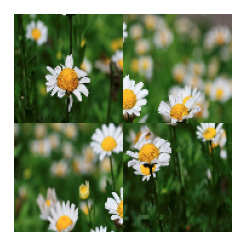
\includegraphics[width=5cm]{images/puzzle}
    \end{subfigure}
    \caption{An example how puzzle for jigsaw pretext task could look like}
\end{figure}

\paragraph{Transfer learning}
For transfer learning EffNet was pre-trained on "imagenette" dataset for image classification.
Imagenete is a selection of 10 classes from the widely known ImageNet dataset. \footnote{
    For information about "imagenette" please refer to \href{https://www.tensorflow.org/datasets/catalog/imagenette}{TF/imagenette}
}

\paragraph{Adversarial Images with FGSM}
My implementation of FGSM was based on \href{https://www.tensorflow.org/tutorials/generative/adversarial_fgsm}{TF FGSM}.
In order to generate adversarial pattern for each image,
gradient of loss function is evaluated with sign for each image.
Then according to this formula:
\begin{equation}
    adv\_x = x + \epsilon \cdot sign(\nabla_x J(\theta, x, y))
\end{equation}
pattern was then added pixel wise to original image with $\epsilon = 0.01$.
Resulting adversarial image was then clipped by value, so each pixel value stays in interval [0\ldots255],
as required for RGB color encoding.

\paragraph{Evaluation approach}
In order to evaluate, how including pretext task in the training process influences NNs vulnerability against adversarial attacks,
I have measured miss-classification rate while keeping the intensity of adversarial pattern fixed at $\epsilon = 0.01$.
\\
Following metrics of interest were recorded:

\begin{equation}
    Accuracy_i = \frac{\# \; images \; correctly \; classified_i}{\# \; test \; images_i} \cdot 100 \%
\end{equation}
\begin{equation}
    \overline{Accuracy} = \frac{1}{N}  \sum_{i=1}^{N}{Accuracy_i}
\end{equation}
\begin{equation}
    Miss \; rate_i = \frac{\# images \; miss \; classified_i}{\# \; images \; correctly \; classified_i} \cdot 100 \%
\end{equation}
\begin{equation}
    \overline{Miss \; rate} = \frac{1}{N}  \sum_{i=1}^{N}{Miss \; rate_i}
\end{equation}
\\
The dataset "tf\_flowers" was chosen for experiment, 5\% of dataset were reserved for evaluation.
\footnote{For information about "tf\_flowers" please refer to \href{https://www.tensorflow.org/datasets/catalog/tf_flowers}{TF/tf\_flowers}}
\\
During each evaluation round NN network was pre-trained either with transfer learning, or rotation, or jigsaw.
The number of training epochs was varied in [15, 30, 45] for pretext training, while the number of epochs for downstream
training was fixed at 30.
\\
Reserved images were given to NN, the correctly classified ones were saved for later use.
Then, for each saved (previously correctly classified) images adversarial example was generated
using FGSM with $\epsilon = 0.01$.
\\
The number of correct classifications, as well as the number of miss-classifications were recorded at the end of each round.

    \section{Methods}

\paragraph{Model}
Convolutional networks' architectures for image recognition have evolved quite drastically in recent years,
with numerous options available "out of the box".
E.g.\ Efficient Net (EffNet) delivers impressive accuracy, while being able to scale better than a lot of
previous architectures~\cite{DBLP:journals/corr/abs-1905-11946}.
For this paper, the evaluation was done using it, namely EfficientNetB0~\cite{KerasEffNet}

\paragraph{Rotation pretext task}
A common choice of pretext task could be to produce 4 copies of
a single image by rotating it by {0°, 90°, 180°, 270°} and let a single network predict the rotation which was applied.
Alexander Kolesnikov and Xiaohua Zhai and Lucas Beyer: "Intuitively, a good model should learn to
recognize canonical orientations of objects in natural images" ~\cite{kolesnikov2019revisiting}.
For this papers evaluation, each image from the original dataset was rotated 0°, 90°, 180°,
270° and assigned a new pseudo label from [0, 1, 2, 3] accordingly.
The examples of such images are shown in~\ref{fig:rot-fig}.
All 4 batches of rotated images, as well as pseudo labels were concatenated in new dataset, and shuffled.
Then EffNet was then trained to identify rotation applied, afterwards the convolutional layers were frozen,
and the output layer size was adjusted for the downstream task \footnote{For details about pretext tasks implementations please refer to
impl/util/pretext.py in accompanying GitHub repository~\cite{github} \label{fn-pre}}.

\begin{figure}[h]
    \begin{subfigure}{0.33\textwidth}
        \caption{Label = 0}
        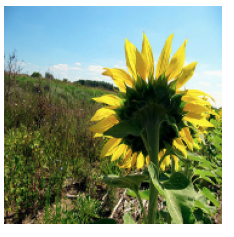
\includegraphics[width=5cm]{images/rot_0}
    \end{subfigure}
    \begin{subfigure}{0.2\textwidth}
        \caption{Label = 1}
        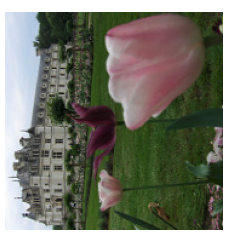
\includegraphics[width=5cm]{images/rot_1}
    \end{subfigure}
    \begin{subfigure}{0.33\textwidth}
        \caption{Label = 2}
        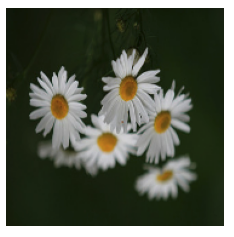
\includegraphics[width=5cm]{images/rot_2}
    \end{subfigure}
    \caption{An example how images used for rotation pretext task could look like}
    \label{fig:rot-fig}
\end{figure}


\paragraph{Jigsaw pretext task}
The task is
to recover relative spatial position of 4 sampled image patches
after a random permutation of these patches was performed
~\cite{kolesnikov2019revisiting}.
All of these patches are concatenated in 'puzzle' image,
which is later sent through the same network, which needs to predict a permutation applied.\
A similar approach as described by Mehdi Noroozi and Paolo Favaro~\cite{DBLP:journals/corr/NorooziF16} was adopted.
Random 4 out of 24 possible permutations were chosen for each batch
(number of possible permutations can be obtained from Newtonian binomial $P=\frac{r!}{(r-n)!}$).
For each permutation, each image was cut in 4 equal parts,
afterwards these tiles were permuted as per chosen permutation, and concatenated in 1 (puzzle) image.
An example can be seen in~\ref{fig:jig-fig}.
Similarly, to rotation pseudo labels in [0\ldots23] had been assigned,
NN was trained to identify permutation applied.
Then the weights of convolutional layers were frozen and reused for the downstream task ^{\ref{fn-pre}}.

\\
\begin{figure}[h]
    \begin{subfigure}{0.33\textwidth}
        \caption{Original image}
        
\includegraphics[width=5cm]{images/dandelion}
    \end{subfigure}
    \begin{subfigure}{0.2\textwidth}
        
\includegraphics[width=3cm]{images/arrow}
    \end{subfigure}
    \begin{subfigure}{0.33\textwidth}
        \caption{Generated puzzle, label=1}
        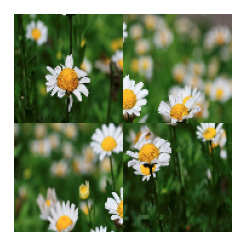
\includegraphics[width=5cm]{images/puzzle}
    \end{subfigure}
    \caption{An example how puzzle for jigsaw pretext task could look like}
    \label{fig:jig-fig}
\end{figure}


\paragraph{Transfer Learning}For this paper, EffNet was pre-trained on "imagenette"~\cite{ImageNette} dataset for image classification.
Imagenette is a subset of 10 easily classified classes from the Imagenet dataset.
Afterwards, the NN was fine-tuned for an actual classification task of interest on~\cite{tfflowers}.

\paragraph{Adversarial Images with FGSM}
The implementation of FGSM for this paper was based on~\cite{FGSM}.
In order to generate an adversarial pattern for each image, as per previously described formula~\ref{eq:adv}
gradient of loss function is evaluated with sign for each image.
Then as per previously described approach,
an adversarial pattern was added pixel wise to the original image with $\epsilon = 0.01$.
The resulting adversarial image was then clipped by value, so each channels' value stays in interval [0\ldots255],
as required for RGB color encoding
\footnote{For details about adversarial attack implementation please refer to
impl/util/adversarial.py in accompanying GitHub repository~\cite{github} \label{fn-adv}}.


\newpage
\paragraph{Evaluation approach}
In order to evaluate, how including pretext task in the training process influences NNs vulnerability against adversarial attacks,
I have measured miss-classification rate while keeping the intensity of adversarial pattern fixed at $\epsilon = 0.01$.
\\
Following metrics of interest were recorded:

\begin{equation}
    Accuracy_i = \frac{\# \; images \; correctly \; classified_i}{\# \; test \; images_i} \cdot 100 \%
\end{equation} \\
where Accuracy\_i is the accuracy in each evaluation round \\
\# stands for "number".

\begin{equation}
    Miss \; rate_i = \frac{\# images \; miss \; classified_i}{\# \; images \; correctly \; classified_i} \cdot 100 \%
\end{equation}
where Miss rate\_i is the miss rate in each evaluation round.


The dataset "tf\_flowers"~\cite{tfflowers} was chosen for experiment, 5\% of dataset were reserved for evaluation.
\\
During each evaluation round NN network was pre-trained either with transfer learning, or rotation, or jigsaw.
The number of training epochs was varied in [15, 30, 45, 60] for pretext training, while the number of epochs for downstream
training was fixed at 30.
\\
The reserved for evaluation images were given to NN. The number of correct classifications was recorded.
Then, for each previously correctly classified image FGSM~\ref{eq:adv} with $\epsilon = 0.01$ was applied.
The number of miss-classifications was recorded afterwards \footnote{For details about evaluation implementations please refer to
impl/util/evaluation.py in accompanying GitHub repository~\cite{github} \label{fn-eval}}.


    \section{Results}

\begin{table}[h]
    \begin{tabular}{|r|r|r|r|}
        \hline
        Pretext epochs & Accuracy, \% & Miss classification rate, \% & $\overline{\epsilon}$ \\
        \hline
        25             & 43.984       & 95.915                       & 0.012                 \\
        50             & 43.438       & 97.482                       & 0.011                 \\
        \rowcolor{yellow}
        75             & 43.281       & 93.141                       & 0.013                 \\
        100            & 42.188       & 95.000                       & 0.012                 \\
        \hline
    \end{tabular}
    \caption{\label{tab:table-1}Results for jigsaw pretext task}
\end{table}



\begin{table}[h]
    \begin{tabular}{|r|r|r|r|}
        \hline
        Pretext epochs & Accuracy, \% & Miss classification rate, \% & $\overline{\epsilon}$ \\
        \hline
        25             & 44.219       & 96.643                       & 0.012                 \\
        50             & 44.141       & 97.876                       & 0.012                 \\
        \rowcolor{yellow}
        75             & 46.953       & 95.674                       & 0.012                 \\
        100            & 44.531       & 97.544                       & 0.012                 \\
        \hline
    \end{tabular}
    \caption{\label{tab:table-2}Results for rotation pretext task}
\end{table}

\begin{table}[h]
    \begin{tabular}{|r|r|r|r|}
        \hline
        Pretext task\textbackslash Pre-training & Accuracy, \% & Miss classification rate, \% & $\overline{\epsilon}$ \\
        \hline
        ImageNet                                & 65.156       & 94.245                       & 0.024                 \\
        None                                    & 39.922       & 99.413                       & 0.011                 \\
        rotation                                & 46.953       & 95.674                       & 0.012                 \\
        jigsaw                                  & 43.984       & 93.141                       & 0.013                 \\
        \hline
    \end{tabular}
    \caption{\label{tab:table-3}Comparison of best results among different pretext tasks, pre-training}
\end{table}

\begin{figure}
    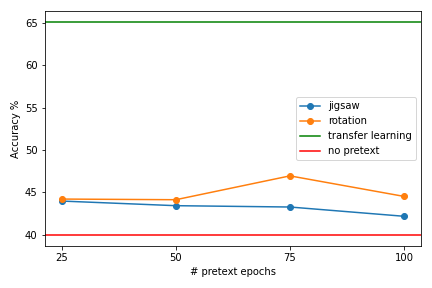
\includegraphics{images/acc}
    \caption{\label{fig:figure-1}Accuracy comparison}
\end{figure}

\begin{figure}
    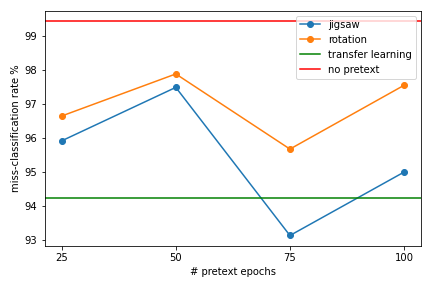
\includegraphics{images/miss_rate}
    \caption{\label{fig:figure-2}Miss rate comparison}
\end{figure}

\begin{figure}
    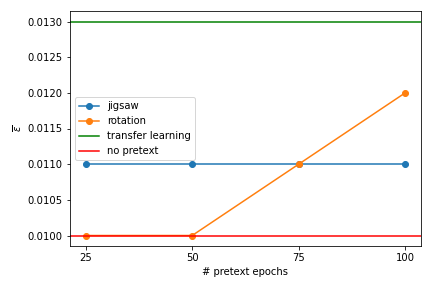
\includegraphics{images/epsilon}
    \caption{\label{fig:figure-3}$\overline{\epsilon}$ comparison}
\end{figure}




    \section{Discussion}

\paragraph{Goal}
In this paper I set up a goal to investigate if including pretext task in training process could reduce NNs
vulnerability against adversarial attacks.

\paragraph{Observations}
\begin{itemize}
    \item both pretext task reduced miss-classification rate a little
    \item both pretext task have improved accuracy a little
    \item accuracy and miss rate are still far from competing with the values for EffNet pre-trained on ImageNet
\end{itemize}

\paragraph{Interpretation}

\paragraph{Limitations}
\begin{itemize}
    \item Evaluation was done only for 1 dataset
    \item Implementation was not peer-reviewed
    \item Hyper parameters of NN (learning-rate, loss function etc.) were not fine-tuned,
    but just taken as recommended from documentation.
\end{itemize}

\paragraph{Conclusion}
Pretext training did give a little improvement in accuracy as well as robustness against adversarial attacks.
However, it's still far from either competing with pre-training on ImageNet or solving the problem of NNs vulnerability
to adversarial attacks.




    \printbibliography
\end{document}
